\section{Charged Pion Identification}

Charged pions are identified and separated from kaons, protons, and electrons
by the amount of energy they lose in the TPC. The dE/dx of a TPC track is
obtained by sorting the track hits according to energy loss, removing the top
30\%, and averaging the rest. Track dE/dx values for a given particle species
at a fixed momentum are Gaussian, so one can also express the dE/dx value for
each track in terms of a deviation from the mean dE/dx for some identified
particle at that track's momentum. In particular, track energy loss values at
STAR are commonly given in terms of ``$n\sigma(\pi)$'', the deviation from the
mean of the pion peak divided by the width of said peak. Protons and kaons
fall to the left of the pion peak (lower energy loss) and electrons fall to
the right (higher energy loss).

The peak position of the raw $n\sigma(\pi)$ distribution generated by the STAR
reconstruction software exhibits some significant time dependence, so instead
of assuming a fixed mean of 0.0 for the pion Gaussian, this analysis performs
a triple Gaussian fit on the $n\sigma(\pi)$ distribution for each fill and
extracts time-dependent means to better calibrate the PID cut. After this
recalibration one can extract yields for the various species of charged
particles by fitting the $n\sigma(\pi)$ distributions with a multi-Gaussian
parametric function. The fitting procedure starts with 8 Gaussians -- one each
for $\pi^{+}$, $\pi^{-}$, $K^{+}$, $K^{-}$, $p$, $\bar{p}$, $e^{+}$, and
$e^{-}$. The number of free parameters is reduced by applying the following
constraints:

\begin{itemize}
    \item all widths must be equal (dE/dx resolution isn't particle-dependent)
    \item particle/antiparticle pairs should have the same mean
    \item $\pi - K$, $\pi - p$, and $\pi - e$ separations are known from other analyses \cite{Xu:2008th}
\end{itemize}

In the end there are 24 - 7 - 4 - 3 = 10 free parameters in the fit: the
Gaussian width, the position of the $\pi$ Gaussian, and the yields. The
particle separations change as a function of momentum, not $p_{T}$, so we
slice a $p_{T}$ bin into momentum bins and fit each one individually. Figure
\ref{fig:typical-nsigmapi} shows a typical fit result. The tracks have been
shifted by 6*charge in order to plot positive and negatively charged tracks on
the same histogram.

\begin{figure}
  \begin{center}
    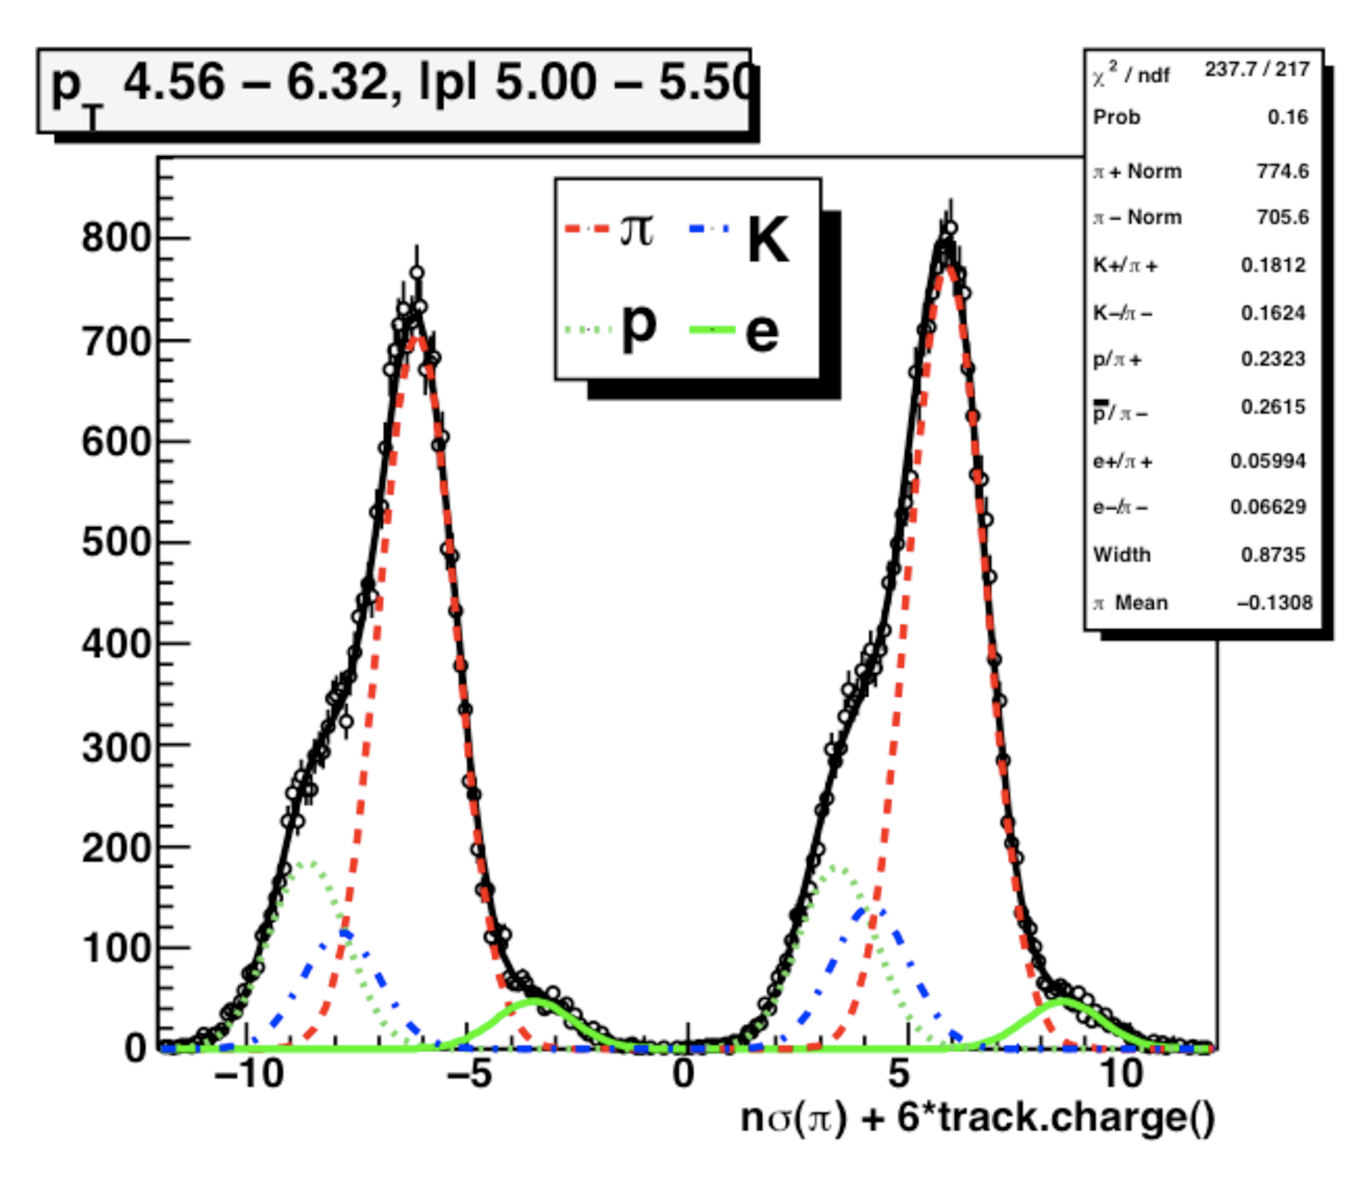
\includegraphics[width=0.7\textwidth]{figures/typical-nsigmapi}    
  \end{center}
  \caption{Example PID fit result}
  \label{fig:typical-nsigmapi}
\end{figure}

With this database of particle yields in hand we can calculate the set of PID
cuts that minimize the statistical uncertainty on the background-subtracted
$A_{LL}$ (Equation \ref{eqn:sigma-all}). A simple minimization routine
assuming $\sigma_{A_{LL}}^{2} = 1/N$ for the raw asymmetries yields the
results in Table \ref{tbl:pid-selection-windows}.

\begin{table}
    \begin{center}
        \begin{tabular}{c|ccc}
        \hline
        $p_{T}$ bin & $\pi$ window & proton/kaon max & electron min\\
        \hline
        \hline
        [2.00 - 3.18] & (-1.10, 2.30) & -2.10 & 2.60\\
        \hline
        [3.18 - 4.56] & (-1.40, 2.10) & -2.10 & 2.40\\
        \hline
        [4.56 - 6.32] & (-1.40, 1.80) & -2.10 & 2.40\\
        \hline
        [6.32 - 8.80] & (-1.40, 1.80) & -2.10 & 2.40\\
        \hline
        [8.80 - 12.84] & (-1.30, 1.40) & -2.10 & 2.10\\
    \hline
    \end{tabular}
    \end{center}
    \caption{PID Selection Windows}
    \label{tbl:pid-selection-windows}
\end{table}
